\chapter[\hspace{0pt}模型建立与求解]{{\heiti\zihao{3}\hspace{0pt}模型建立与求解}}\label{chapter3: 模型建立与求解}
\removelofgap
\removelotgap

\section[\hspace{-2pt}问题1:颜色空间转换模型]{{\heiti\zihao{-3} \hspace{-8pt}问题1:颜色空间转换模型}}\label{section3: 问题1:颜色空间转换模型}

\subsection[\hspace{-2pt}模型建立与求解]{{\heiti\zihao{4} \hspace{-8pt}模型建立与求解}}\label{section3: 模型建立与求解}

% \noindent\textbf{优化方法与数学建模}

为求解 BT.2020 空间到显示屏 RGB 空间的最优线性映射矩阵 $M\in \mathbf{R}^{3\times 3}$,我们采样一组代表性 BT.2020 RGB 样本 $\{c_{i}\}_{i=1}^{N}\in [0,1]^{3}$,其色彩向量经过如下映射:
\begin{equation}\label{eq:linear_map}
  c^{'}_{i} = M\,c_{i}
\end{equation}
然后通过预定义的色彩转换矩阵 $M_{BT\rightarrow XYZ}$ 与 $M_{DP\rightarrow XYZ}$ 将源与目标向量映射至 XYZ 空间,并进一步转换至 CIELab 空间,计算感知误差 $\Delta E_{00}$:
\begin{equation}\label{eq:deltaE}
  L(M)=\frac{1}{N}\sum_{i=1}^{N}\Delta E_{00}\bigl(\mathrm{Lab}(M_{BT\rightarrow XYZ}\,c_{i}),\;\mathrm{Lab}(M_{DP\rightarrow XYZ}\,M\,c_{i})\bigr).
\end{equation}

优化目标为:
\begin{equation}\label{eq:opt_obj}
  \underset {M\in \mathbb{R}^{3\times 3}}{\min}\;L(M).
\end{equation}

为求解上述非线性、不可导且可能存在多个局部极小值的优化问题,我们引入差分进化 (Differential Evolution, DE) 算法。DE 算法以种群为基础,通过变异、交叉和选择操作迭代更新种群,逐步逼近最优解。

\noindent\textbf{(1)参数编码与搜索空间}\
将 $M$ 展开为 9 维向量 $\mathbf{x}=\mathrm{vec}(M)\in \mathbb{R}^9$,定义每维搜索空间边界为:
\begin{equation}\label{eq:search_space}
  x_{j}\in [l_j, u_j]=[-2,2],\quad j=1,\dots,9.
\end{equation}

\noindent\textbf{(2)初始化种群}\
生成种群大小为 $NP$ 的初始个体 $\{\mathbf{x}_i^{(0)}\}_{i=1}^{NP}$:
\begin{equation}\label{eq:init_pop}
  x^{(0)}_{i,j} = l_j + r_{i,j}(u_j - l_j),\quad r_{i,j}\sim\mathcal{U}(0,1).
\end{equation}

\noindent\textbf{(3)变异操作}\
对第 $i$ 个个体,在种群中随机选择三个不同的个体 $\mathbf{x}_{r1}, \mathbf{x}_{r2}, \mathbf{x}_{r3}$,构造变异向量:
\begin{equation}\label{eq:mutation}
  \mathbf{v}_i^{(t)} = \mathbf{x}_{r1}^{(t)} + F\bigl(\mathbf{x}_{r2}^{(t)} - \mathbf{x}_{r3}^{(t)}\bigr),
\end{equation}
其中 $F\in (0,2)$ 为差分缩放因子。

\noindent\textbf{(4)交叉操作}\
根据交叉概率 $CR\in [0,1]$ 构造试验向量 $\mathbf{u}_i^{(t)}$:
\begin{equation}\label{eq:crossover}
  u_{i,j}^{(t)} =
  \begin{cases}
    v_{i,j}^{(t)},&\text{if } \mathrm{rand}_j\le CR\text{ or } j=j_{rand},\\
    x_{i,j}^{(t)},&\text{otherwise},
  \end{cases}
\end{equation}
其中 $\mathrm{rand}_j\sim\mathcal{U}(0,1)$ 且 $j_{rand}$ 确保至少一维来自 $\mathbf{v}_i^{(t)}$。

\noindent\textbf{(5)选择操作}\
将试验向量 $\mathbf{u}_i^{(t)}$ 和当前个体 $\mathbf{x}_i^{(t)}$ 对应的映射矩阵 $M=\mathrm{mat}(\cdot)$ 代入目标函数 $L$,保留更优者:
\begin{equation}\label{eq:selection}
  \mathbf{x}_i^{(t+1)} =
  \begin{cases}
    \mathbf{u}_i^{(t)},&\text{if } L\bigl(\mathrm{mat}(\mathbf{u}_i^{(t)})\bigr)<L\bigl(\mathrm{mat}(\mathbf{x}_i^{(t)})\bigr),\\
    \mathbf{x}_i^{(t)},&\text{otherwise}.
  \end{cases}
\end{equation}

其中,$L(\mathrm{mat}(\mathbf{x}))$ 由式(\ref{eq:deltaE}) 计算。

\noindent\textbf{(6)终止条件}\
满足以下任一条件则终止迭代:
\begin{itemize}
  \item 最大迭代代数 $T_{max}$;
  \item 种群最优个体的目标函数值变化小于阈值 $\epsilon$。
\end{itemize}

最终输出最优映射矩阵 $M^*=\mathrm{mat}(\mathbf{x}_{best})$,其中
\begin{equation}\label{eq:best_solution}
  \mathbf{x}_{best} = \arg\min_{i=1,\dots,NP} L\bigl(\mathrm{mat}(\mathbf{x}_i^{(T)})\bigr).
\end{equation}


综上所述,为优化色彩转换矩阵 $M$,本文选用差分进化算法(DE)。该方法将 $M$ 参数化为9维向量,并在预设的搜索空间边界内进行优化。通过其经典的种群初始化、变异、交叉及选择等核心操作,DE算法能够迭代地搜寻旨在最小化以 $\Delta E_{00}$ 度量的感知色彩差异的解。鉴于目标函数的非线性、不可导以及可能存在多个局部极小值的特性,DE算法的全局优化能力和鲁棒性,使其成为获取高质量色彩映射的有效计算途径。

% \noindent\textbf{差分进化算法(Differential Evolution, DE)}

\subsection[\hspace{-2pt}问题一结果分析]{{\heiti\zihao{4} \hspace{-8pt}问题一结果分析}}\label{section4: 问题一结果分析}


为实现 BT.2020 色域向目标显示屏 RGB 色域的最优映射,本文构建了感知误差最小化的优化模型,目标为在 CIELab 空间中最小化 $\Delta E_{00}$ 感知色差。我们采样了多个 BT.2020 RGB颜色点,并通过线性映射矩阵 $M\in \mathbb{R}^{3\times 3}$ 变换后,转化至目标显示屏空间,再经过标准变换矩阵应设至 XYZ、CIELab 空间,并利用 $\Delta E_{00}$ 公式计算感知误差。

在模型求解过程中,本文采用了差分进化(Differential Evolution, DE)优化方法,对初始映射矩阵进行迭代寻优。为验证我们模型的稳定性,并提供更可靠的性能评价,我们执行了 50 轮随机优化,并统计其性能指标。主要分析结果如下:

\noindent\textbf{(1)$\Delta E_{00}$感知误差分布}

图 1 显示了在50次独立优化实验中,各次优化所达成的最终 $\Delta E_{00}$ 损失值分布情况。其中最大值为 1.0183 ,这表明映射结果在感知层面极为接近参考目标。均值为 0.0744 ,标准差为 0.2083 。这表明该基于 $\Delta E_{00}$ 损失函数的差分进化算法在不同采样条件下都能稳定收敛于较小的感知误差区域,并且具有良好的泛化性能以及良好的稳定性和鲁棒性。
\begin{figure}[h]
\centering
\captionsetup{font={small, stretch=1.312}}
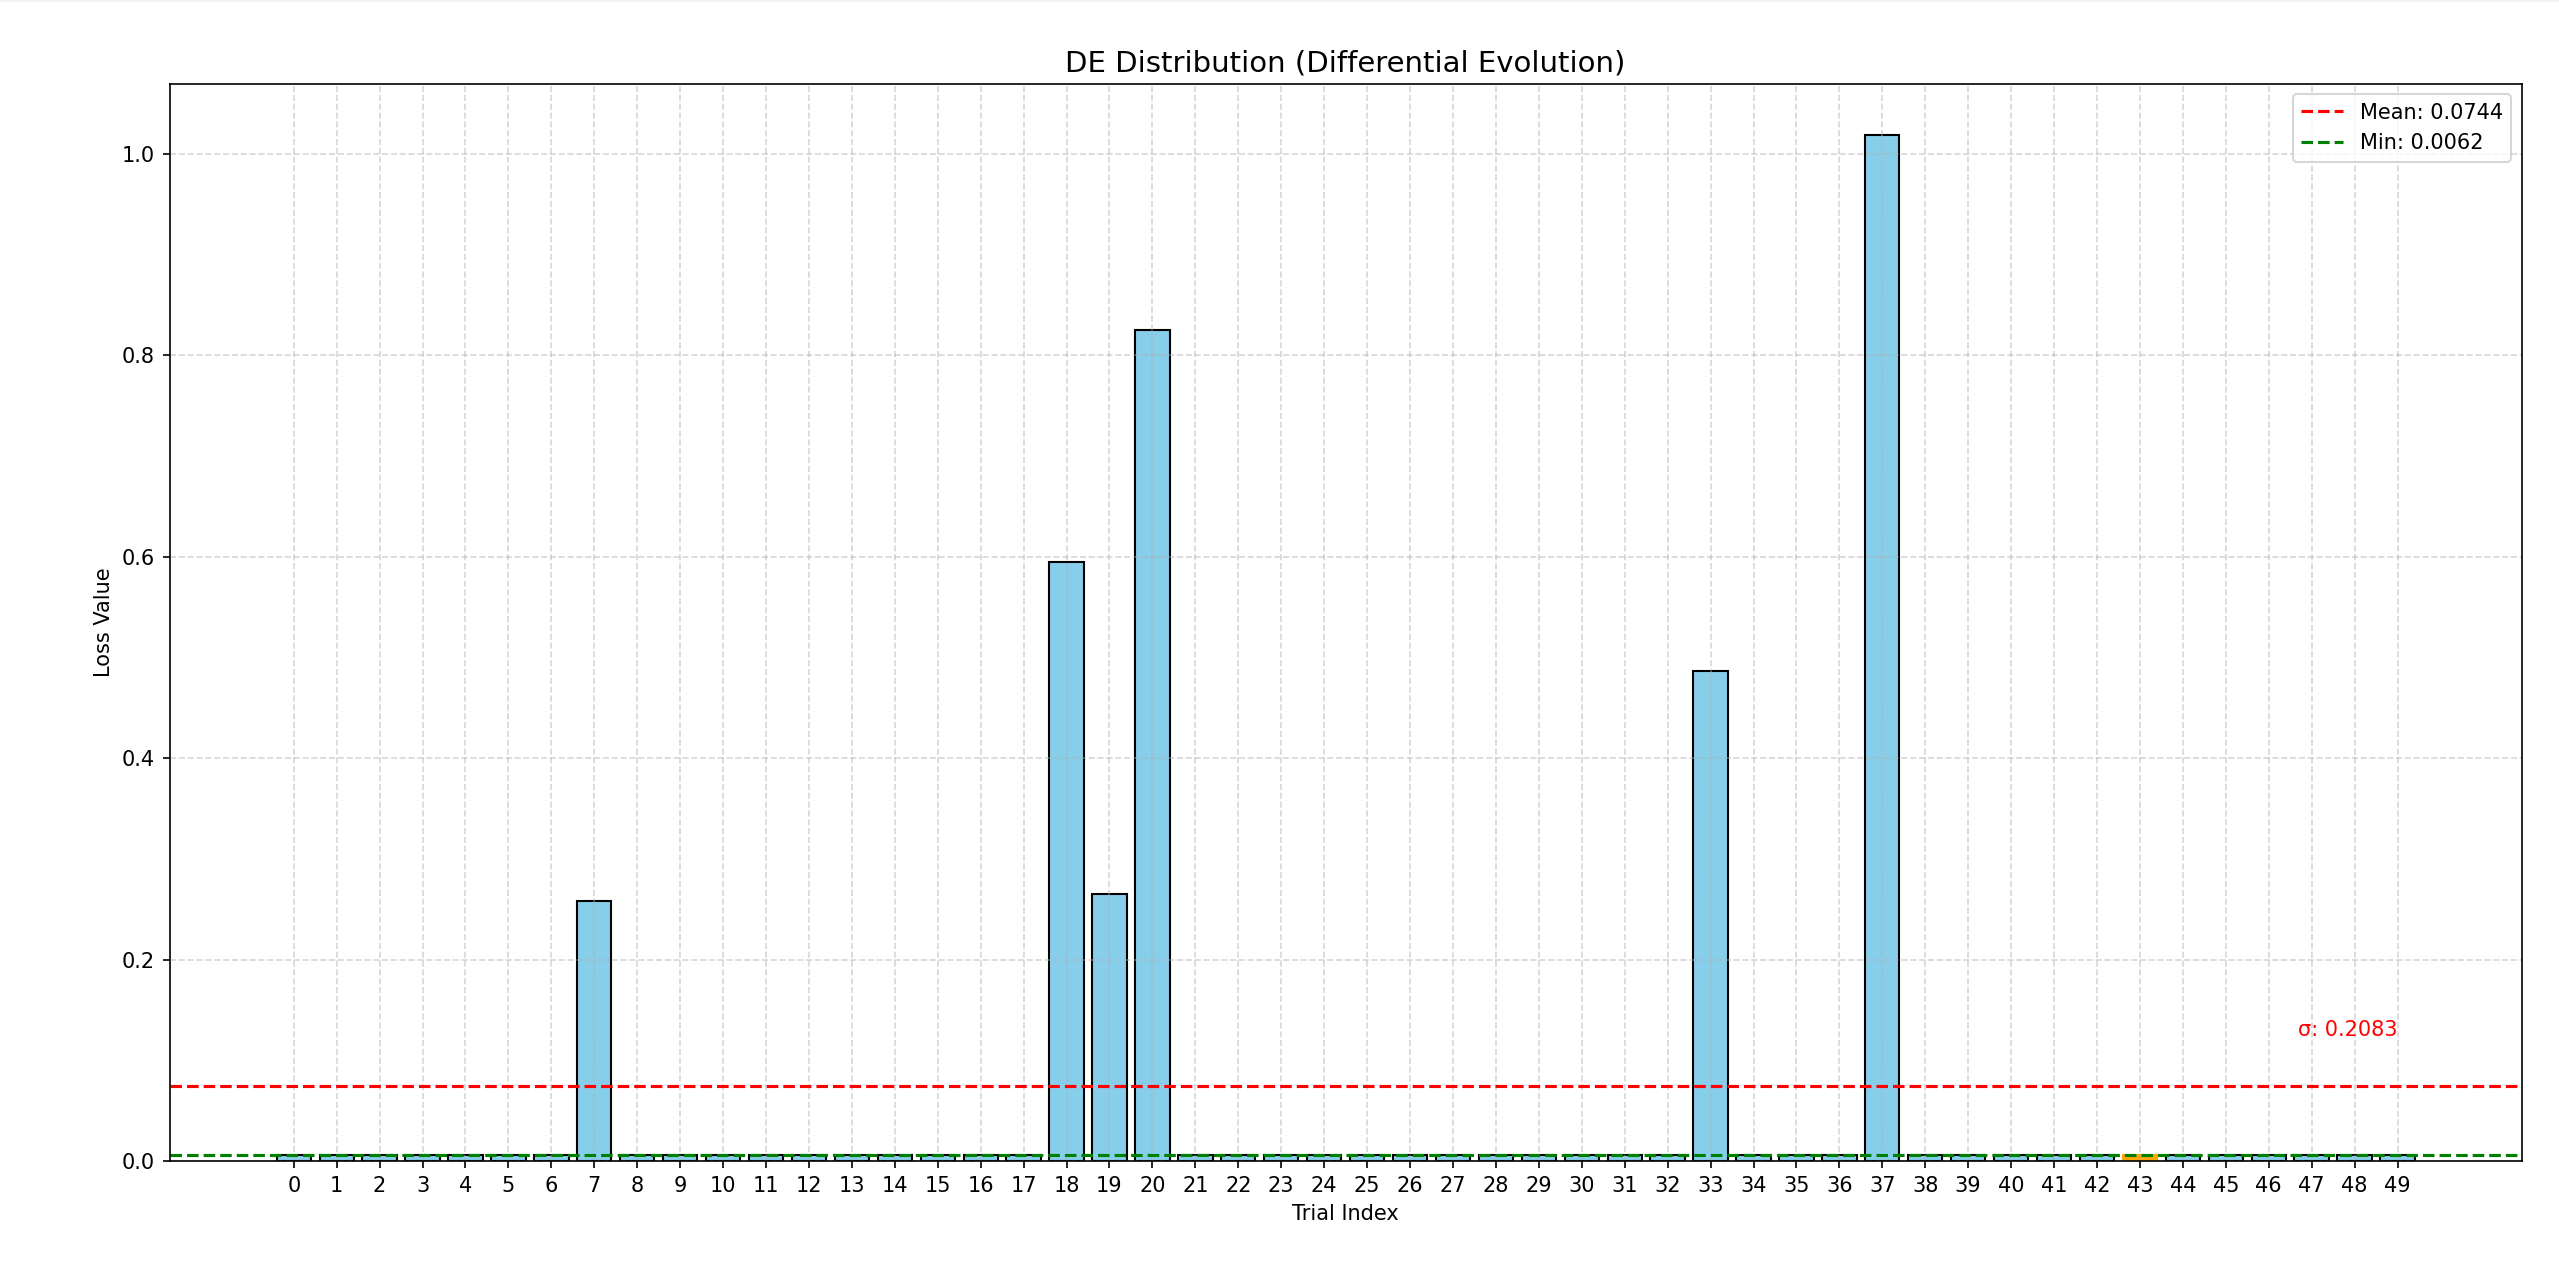
\includegraphics[width=1.0\columnwidth]{figures/DE2000.png}
% \captionsetup{justification=justified,singlelinecheck=false}
\bicaption[50次独立优化实验柱状损失图]{}[]{}
\vspace{-10pt}
\label{figure3: 柱状loss}
\end{figure}

\noindent\textbf{(2)色度空间三角形面积变化}

为评估映射后色域覆盖度变化,我们进一步对比了sRGB 色度三角与模型输出映射后所得的色度三角面积。面积通过三角形在 CIE xy 色度图上的顶点(RGB 基色经映射后的 xy 坐标)计算而得。结果表明,所有 50 次优化中,面积差绝对值均低于 0.001,说明映射后色域几乎无压缩,色彩覆盖极小损失。
\begin{figure}[htbp]
\centering
\captionsetup{font={small, stretch=1.0}}
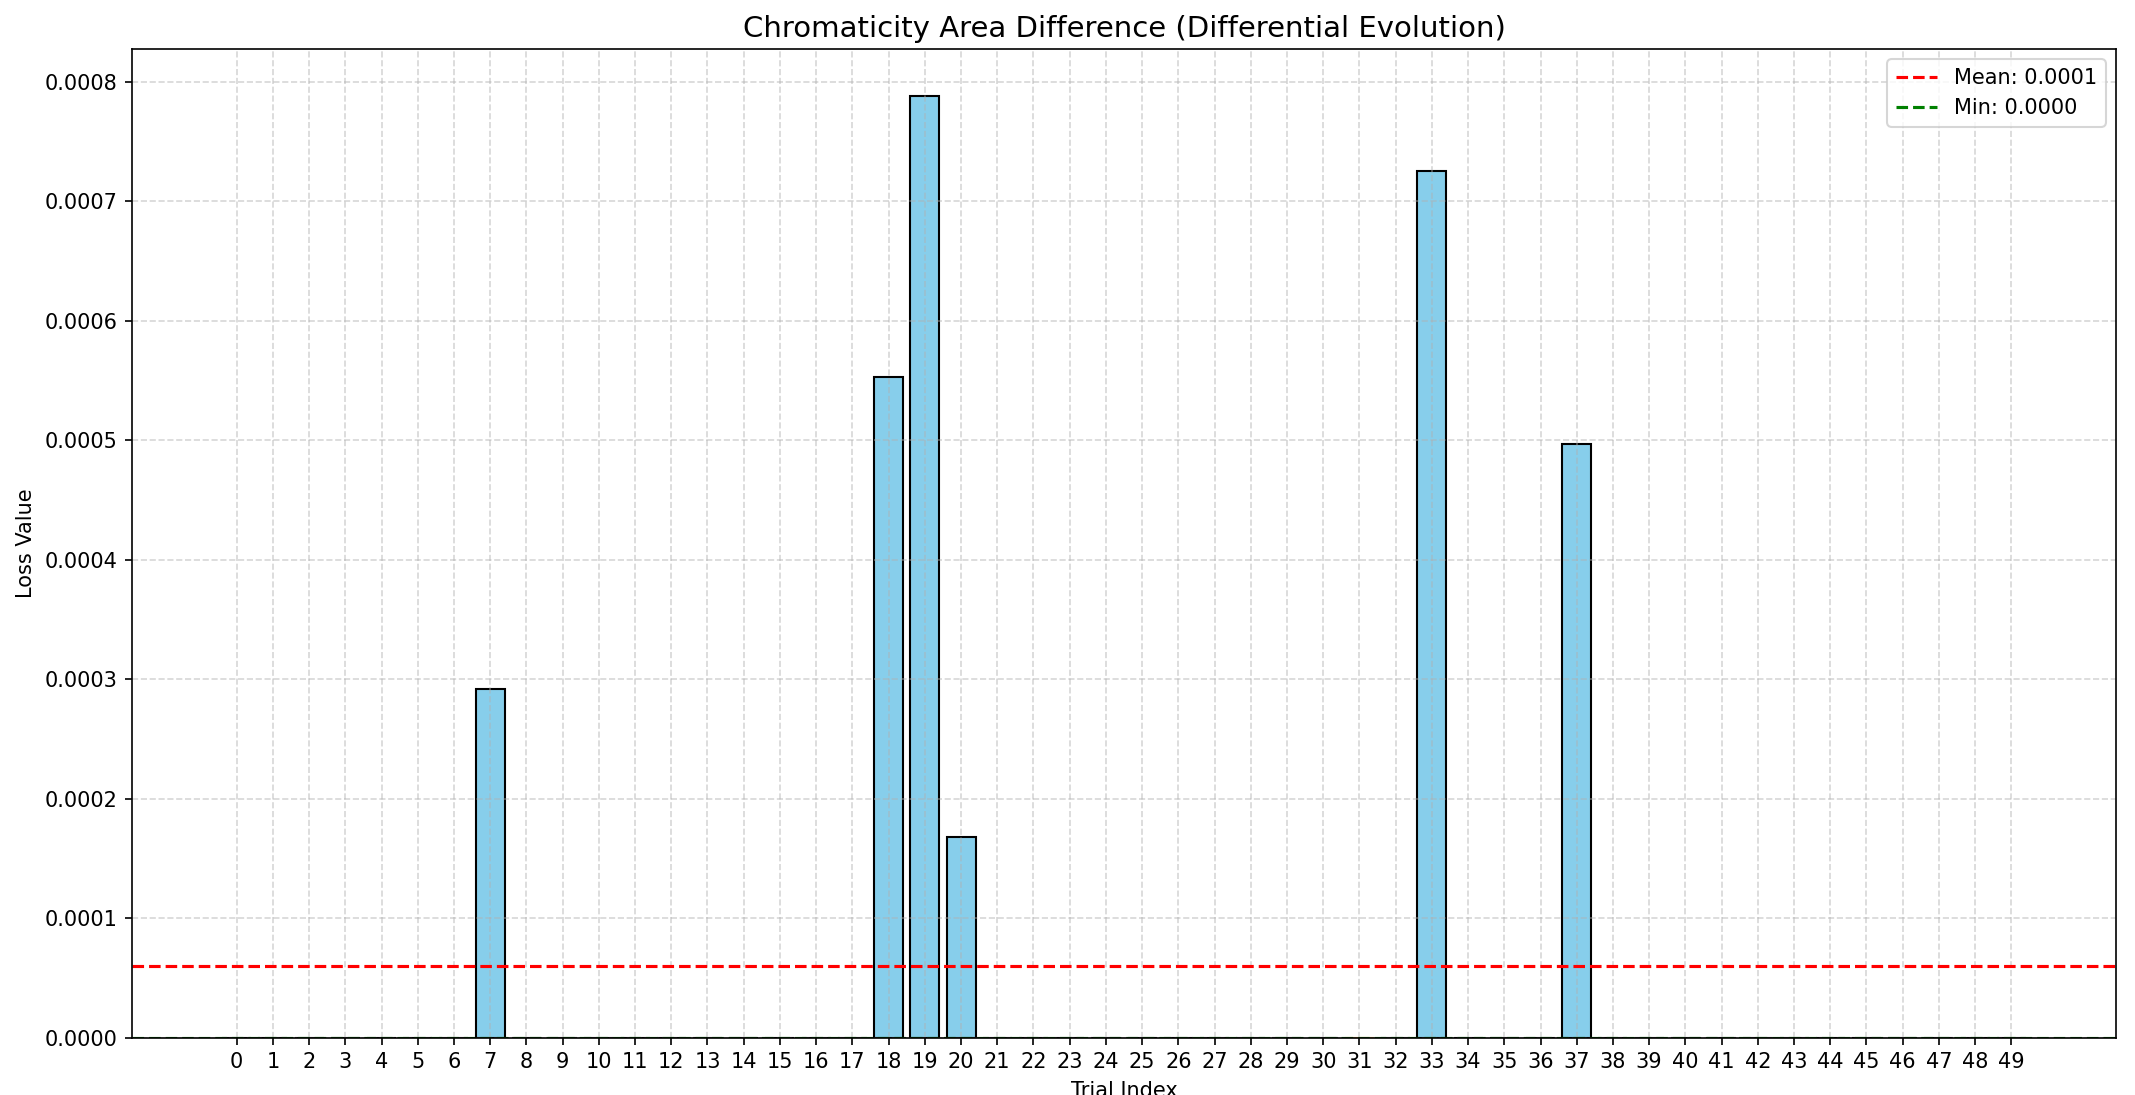
\includegraphics[width=0.8\columnwidth]{figures/面积Loss.png}
% \captionsetup{justification=justified,singlelinecheck=false}
\bicaption[50次独立优化实验面积差图]{}[]{}
\vspace{-10pt}
\label{figure3: 面积diff}
\end{figure}
显然我们可以得出,模型在保持色域范围完整性的同时,完成了精准的 RGB 空间映射,并且与 sRGB 的覆盖几乎一致,无明显压缩或扭曲现象。映射后的面积误差控制在 $10^{-3}$ 量级,说明模型不仅保持了色彩准确性,也很好地保留了 BT.2020 色域映射后的覆盖特性。

\noindent\textbf{(3)色度图可视化对比}

为直观评估映射效果,我们将 BT.2020、sRGB 以及映射后所得色度三角同时绘制于 CIE 1931 xy 色度图中(见图 3)。可以观察到,模型优化后所得色度三角与标准 sRGB 色域几乎完全重合,进一步验证了在极低感知误差下,实现了对目标色域的高保真拟合。
\begin{figure}[h]
\centering
\captionsetup{font={small, stretch=1.0}}
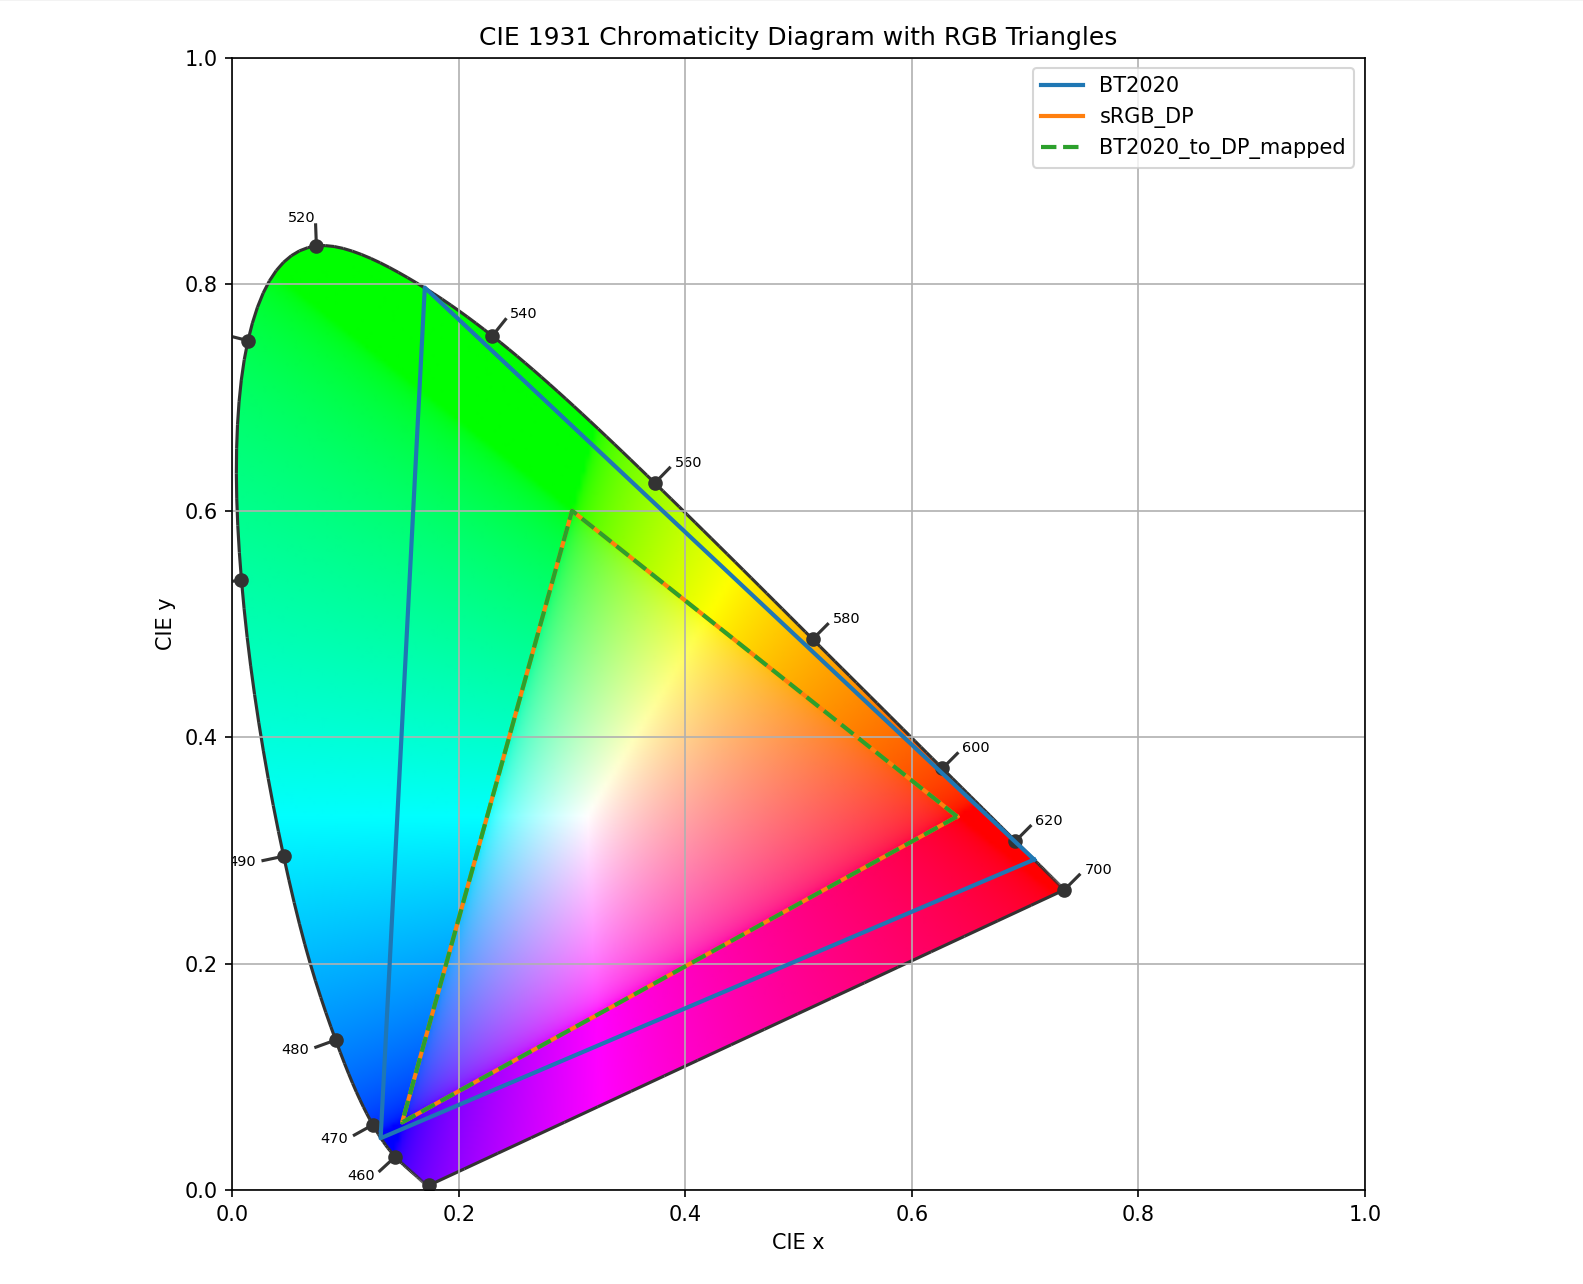
\includegraphics[width=0.8\columnwidth]{figures/色度.png}
% \captionsetup{justification=justified,singlelinecheck=false}
\bicaption[色度图]{}[]{}
\vspace{-10pt}
\label{figure3: 色度图}
\end{figure}


\section[\hspace{-2pt}问题2:四通道到五通道颜色转换模型]{{\heiti\zihao{-3} \hspace{-8pt}问题2:四通道到五通道颜色转换模型}}\label{section3: 问题2:四通道到五通道颜色转换模型}
\subsection[\hspace{-2pt}问题分析与建模目标]{{\heiti\zihao{4} \hspace{-8pt}问题分析与建模目标}}\label{section2: 问题分析与建模目标}

本问题旨在解决从 4 通道相机 (RGBV) 到 5 通道 LED 显示屏 (RGBCX) 的颜色空间转换问题。其核心挑战在于:
\begin{enumerate}
    \item \textbf{通道数量不匹配}:输入是 4 维,输出是 5 维。这意味着简单的线性变换可能无法有效完成映射,且需要模型能够“创造”出多余的输出通道信息。
    \item \textbf{非线性转换}:相机捕捉到的 RGBV 信号与显示屏所需的 RGBCX 信号之间通常存在复杂的非线性关系,这可能源于设备响应曲线、环境光照、传感器特性以及显示屏自身的物理特性。
    \item \textbf{最小化感知差异}:转换后的颜色应尽可能保留原始颜色的人眼感知,即 $\Delta E_{2000}$ 应尽可能小。这是衡量颜色转换质量的关键指标,简单地最小化数值误差可能无法保证视觉效果。
\end{enumerate}

因此,我们的建模目标是建立一个能够将 4 维相机输入(RGBV)映射到 5 维显示输出(RGBCX)的非线性模型,并以最小化颜色感知差异(即 $\Delta E_{2000}$)为主要优化目标,同时保证输出值在合理的物理范围内。

\subsection[\hspace{-2pt}神经网络模型:ColorNet 的设计与原理]{{\heiti\zihao{4} \hspace{-8pt}神经网络模型:ColorNet 的设计与原理}}\label{section2: 神经网络模型}

鉴于颜色空间转换的复杂非线性特性,以及输入输出维度不匹配的问题,我们选择使用\textbf{前馈神经网络 (Feedforward Neural Network, FNN)} 来作为主要的映射模型。FNN 具有强大的非线性拟合能力,能够学习并逼近任意复杂的函数关系,非常适合此类多输入多输出的映射问题。

\textbf{模型结构 (ColorNet):}

我们设计了一个包含多个全连接层(也称为线性层)的神经网络,其结构如下:

\begin{itemize}
    \item \textbf{输入层 (Input Layer)}:
        \begin{itemize}
            \item 包含 \textbf{4 个神经元}。
            \item 每个神经元对应相机捕捉到的一个颜色通道值:红 (R), 绿 (G), 蓝 (B), 以及额外的 V (假设为某种光谱以外的特殊通道或相机特定校准通道)。
            \item 输入数据直接传入,不进行激活函数处理。
        \end{itemize}
    \item \textbf{隐藏层 (Hidden Layers)}:
        \begin{itemize}
            \item 本模型采用了 \textbf{3 个隐藏层},以提供足够的模型容量来学习复杂的非线性映射。
            \item \textbf{第一隐藏层}:将 4 维输入映射到 64 维特征空间。ReLU (Rectified Linear Unit) 激活函数 $f(x) = \max(0, x)$ 引入了非线性,使得网络能够学习到非线性特征。
            \item \textbf{第二隐藏层}:进一步将特征维度提升至 128 维。增加维度有助于网络发现更丰富的特征组合。
            \item \textbf{第三隐藏层}:将特征维度降回 64 维。这种“宽-窄”结构有助于信息在不同抽象层次上的流动和提炼。
        \end{itemize}
    \item \textbf{输出层 (Output Layer)}:
        \begin{itemize}
            \item 包含 \textbf{5 个神经元},对应 LED 显示屏的五个输出通道:红 (R), 绿 (G), 蓝 (B), 青 (C), 以及额外的 X (假设为一种补充红色或特定效果通道)。
            \item `Sigmoid` 激活函数 $f(x) = \frac{1}{1+e^{-x}}$ 将输出值限制在 \textbf{[0, 1]} 范围内。这是至关重要的,因为颜色通道值通常表示强度或亮度,必须是非负且有上限的。Sigmoid 函数保证了输出的物理合理性,避免了负值或过大值,这对于后续的颜色空间转换(如 RGB 到 Lab)也是必需的。
        \end{itemize}
\end{itemize}

选择 FNN 的优势在于其灵活性和通用性。无需对输入输出关系进行复杂的先验假设,FNN 可以通过训练自动从数据中学习到最佳的映射方式。多层结构和非线性激活函数使其能够处理高度复杂的颜色转换曲线和相互作用。

\subsection[\hspace{-2pt}损失函数设计:混合损失的哲学与实现]{{\heiti\zihao{4} \hspace{-8pt}损失函数设计:混合损失的哲学与实现}}\label{section2: 损失函数设计}

为了实现模型“最小化感知差异”的核心目标,我们设计了一个\textbf{混合损失函数 (Combined Loss)}。这个损失函数融合了两种不同的误差度量,旨在同时满足数值准确性和视觉准确性。

\subsubsection[\hspace{-2pt}均方误差 (Mean Squared Error, MSE) Loss]{{\heiti\zihao{4} \hspace{-8pt}均方误差 (Mean Squared Error, MSE) Loss}}\label{section2: MSE Loss}

\begin{itemize}
    \item \textbf{定义}:
    $ L_{MSE} = \frac{1}{N} \sum_{i=1}^N \| \text{pred\_rgbcx}_i - \text{target\_rgbcx}_i \|^2 $
    其中,$N$ 是样本数量,$\text{pred\_rgbcx}_i$ 是模型对第 $i$ 个样本的 5 通道预测输出,$\text{target\_rgbcx}_i$ 是第 $i$ 个样本的真实 5 通道目标输出。$\| \cdot \|^2$ 表示欧氏距离的平方。
    \item \textbf{作用}:MSE 是一种普遍使用的回归损失,它惩罚了预测值与目标值之间的数值差异。在颜色转换中,MSE 确保了模型在所有 5 个输出通道上的数值接近目标值。它有助于网络的稳定训练,防止输出值出现极端或不合理的波动,并为后续的颜色空间转换(如 RGB 到 Lab)提供一个稳固的基础。它在一定程度上反映了能量或信号强度的匹配。
\end{itemize}

\subsubsection[\hspace{-2pt}$\Delta E_{2000}$ Loss (感知误差)]{{\heiti\zihao{4} \hspace{-8pt}$\Delta E_{2000}$ Loss (感知误差)}}\label{section2: Delta E 2000 Loss}

\begin{itemize}
    \item \textbf{定义}:
    $ L_{\Delta E_{2000}} = \frac{1}{N} \sum_{i=1}^N \Delta E_{2000}(\text{pred\_lab}_i, \text{target\_lab}_i) $
    这里,$\text{pred\_lab}_i$ 是将模型预测的 RGBCX 输出中的 \textbf{RGB 部分} 转换到 Lab 颜色空间的结果,而 $\text{target\_lab}_i$ 则是将真实 RGBCX 目标中的 \textbf{RGB 部分} 转换到 Lab 颜色空间的结果。
    \item \textbf{转换过程 (PyTorch 实现)}:
        \begin{itemize}
            \item \textbf{sRGB RGB to XYZ}:首先,将 sRGB 空间下的 RGB 值(限制在 [0,1] 范围内)转换为线性 RGB 值,然后通过一个 3x3 的转换矩阵 $M_{sRGB \to XYZ}$ 得到 XYZ 空间坐标。
            \item \textbf{XYZ to Lab}:接着,将 XYZ 坐标(经过白点归一化)转换为 Lab 坐标。这个转换涉及非线性函数 $f(t)$,用于模拟人眼对亮度的非线性感知。
            \item \textbf{Delta E 2000}:最后,使用 PyTorch 实现的 $\Delta E_{2000}$ 公式计算预测 Lab 值与目标 Lab 值之间的颜色差异。这个公式非常复杂,涉及到多种修正项(如亮度、彩度、色调的权重,以及旋转项),以更准确地反映人眼的感知非线性。 
        \end{itemize}
    \item \textbf{作用}:$L_{\Delta E_{2000}}$ 是本模型的核心创新点,因为它直接优化了人眼感知的颜色差异。相比于 MSE 仅关注数值上的匹配,$\Delta E_{2000}$ 损失能够引导模型生成在视觉上更接近目标颜色的输出。通过最小化这个损失,即使数值上存在细微差异,只要它们在感知上是难以区分的,模型也会认为这是良好的结果。
\end{itemize}

\subsubsection[\hspace{-2pt}总损失函数 (Total Loss)]{{\heiti\zihao{4} \hspace{-8pt}总损失函数 (Total Loss)}}\label{section2: Total Loss}

\begin{itemize}
    \item \textbf{组合}:
    $ L_{total} = \alpha \cdot L_{MSE} + \beta \cdot L_{\Delta E_{2000}} $
    \item \textbf{权重选择}:在代码中,我们设置了 \textbf{$\alpha=0.1$ 和 $\beta=1.0$}。
        \begin{itemize}
            \item \textbf{更高的 $\beta$ 值 (1.0)}:这表明我们赋予 $\Delta E_{2000}$ 损失更高的权重,明确指出我们优先考虑颜色转换的感知准确性。这是因为在颜色重现任务中,人眼的视觉效果往往比像素值的绝对数值更重要。
            \item \textbf{较低的 $\alpha$ 值 (0.1)}:虽然 $\Delta E_{2000}$ 是主要目标,但保留一定比例的 MSE 损失仍然有益。MSE 损失可以提供一个更平滑的优化曲面,帮助模型在训练初期快速收敛,并避免某些极端情况下的数值不稳定。它也确保了模型在非 RGB 通道(C 和 X)上的数值合理性,因为 $\Delta E_{2000}$ 仅针对 RGB 部分。
        \end{itemize}
    \item \textbf{平衡}:通过调整 $\alpha$ 和 $\beta$,可以在数值精确度和感知准确度之间找到最佳平衡点。这个平衡点通常需要根据具体的应用场景和视觉要求进行实验和调整。
\end{itemize}

\subsection[\hspace{-2pt}数据生成与训练策略]{{\heiti\zihao{4} \hspace{-8pt}数据生成与训练策略}}\label{section2: 数据生成与训练策略}

由于实际的 4 通道相机和 5 通道显示屏数据通常难以获取,我们采用了\textbf{模拟数据生成}的方法。这种方法允许我们创建足够多样化的训练样本,以训练神经网络学习复杂的映射关系。

\subsubsection[\hspace{-2pt}训练数据生成]{{\heiti\zihao{4} \hspace{-8pt}训练数据生成}}\label{section2: 训练数据生成}

\begin{itemize}
    \item \textbf{输入数据 $X$ (RGBV)}:
        \begin{itemize}
            \item 随机生成 `$n_samples$` (例如 4000) 个样本,每个样本包含 4 个通道的值。
            \item 每个通道的值都在 `[0, 1]` 范围内均匀随机分布。
            \item 这模拟了相机在各种亮度(R, G, B)和特殊通道 (V) 下可能捕捉到的信号。
        \end{itemize}
    \item \textbf{目标数据 $Y$ (RGBCX)}:
        \begin{itemize}
            \item 目标数据的生成旨在模拟一个相对复杂但可控的真实世界颜色转换。
            \item 首先,通过一个预设的 \textbf{线性变换矩阵 $W$} 对输入 $X$ 进行加权乘法,得到线性输出 $Y_{linear}$。这个矩阵 $W$ 定义了 RGBV 到 RGBCX 的基础线性映射。
                这种交叉影响模拟了真实世界颜色混合的复杂性,例如,一个输入通道可能不仅仅影响对应的输出通道,还会微弱影响其他输出通道,这在多光谱成像和显示系统中很常见。
            \item 接着,在 $Y_{linear}$ 的基础上添加一个\textbf{非线性扰动} 。
                \begin{itemize}
                    \item 这个扰动项是基于输入 R 通道 的一个正弦函数,并带有较小的幅度 (0.02)。
                    \item $5 \pi X$ 使得正弦波在 [0,1] 范围内有 2.5 个周期,这意味着引入的非线性变化是非单调的,能够更好地模拟真实设备响应中的非线性效应,例如,某些颜色通道在特定输入强度下可能表现出非线性的响应,或者存在一些难以用简单线性模型捕捉的串扰。引入这种非线性扰动,迫使神经网络学习更复杂的映射,而不仅仅是简单的线性变换。
                \end{itemize}
            \item 最后,将所有输出值 \textbf{裁剪到 [0, 1] 范围}。这是为了确保颜色通道值保持在物理上合理的范围内,因为颜色通常被归一化到这个范围,超出此范围的值没有物理意义。
        \end{itemize}
\end{itemize}

\subsubsection[\hspace{-2pt}训练策略]{{\heiti\zihao{4} \hspace{-8pt}训练策略}}\label{section2: 训练策略}

\begin{itemize}
    \item \textbf{优化器}:选用 \textbf{AdamW} 优化器。AdamW 是 Adam 优化器的一种改进版本,它在权重衰减(L2 正则化)的处理上更为有效,有助于防止过拟合,并提高模型在训练过程中的稳定性。
    \item \textbf{学习率 (Learning Rate)}:设置为 $5 \times 10^{-4}$。这个学习率是一个常用的起始值,它足够小以避免训练发散,又足够大以保证合理的收敛速度。
    \item \textbf{训练集-验证集划分}:
        \begin{itemize}
            \item 将生成的总数据集按 80\% 训练集和 20\% 验证集进行划分 (\texttt{test\_size=0.2}, \texttt{random\_state=42}确保可复现性)。
            \item 训练集用于模型的参数更新。
            \item 验证集用于在训练过程中评估模型的泛化能力。在每个 epoch 结束后,模型会在验证集上计算损失,这个损失不参与模型的参数更新,但可以用于监控模型是否过拟合(即训练损失持续下降而验证损失开始上升)。
        \end{itemize}
    \item \textbf{批次训练 (Batch Training)}:
        \begin{itemize}
            \item 训练数据在每个 epoch 开始前会进行随机打乱。
            \item 训练过程以小批量 (batch size=32) 的方式进行。批次训练有多个优点:
                \begin{itemize}
                    \item \textbf{提高训练效率}:每次迭代处理少量数据,而不是整个数据集,可以更快地进行参数更新。
                    \item \textbf{平滑梯度}:每次迭代的梯度是基于一个小批量的平均值,这有助于减小梯度估计的方差,使训练过程更稳定。
                    \item \textbf{防止过拟合}:引入一定的随机性,有助于模型更好地泛化。
                \end{itemize}
        \end{itemize}
    \item \textbf{设备选择}:模型训练会优先使用 GPU ("cuda") 如果可用,否则退回到 CPU ("cpu")。GPU 能够显著加速深度学习模型的训练过程。
    \item \textbf{监控与报告}:在训练过程中,每隔一定 epoch(例如每 10 个 epoch)会打印当前的训练损失和验证损失,以便实时监控模型的学习进度和性能。
\end{itemize}

通过上述详细的模型建立和解析,我们不仅明确了模型的基本架构和关键组成部分,更深入地探讨了其设计哲学和每个组件在解决颜色空间转换问题中的作用,尤其是混合损失函数在平衡数值和感知准确性方面的核心价值。

\section[\hspace{-2pt}模型求解和结果分析]{{\heiti\zihao{-3} \hspace{-8pt}模型求解和结果分析}}\label{section2: 模型求解和结果分析}

\subsection[\hspace{-2pt}训练过程与损失曲线]{{\heiti\zihao{4} \hspace{-8pt}训练过程与损失曲线}}\label{section2: 训练过程与损失曲线}

通过运行提供的 Python 代码,我们训练了 ColorNet 模型。训练损失曲线展示了模型在训练集和验证集上的收敛情况。



\begin{figure}[h!]
\centering
\captionsetup{font={small, stretch=1.312}}
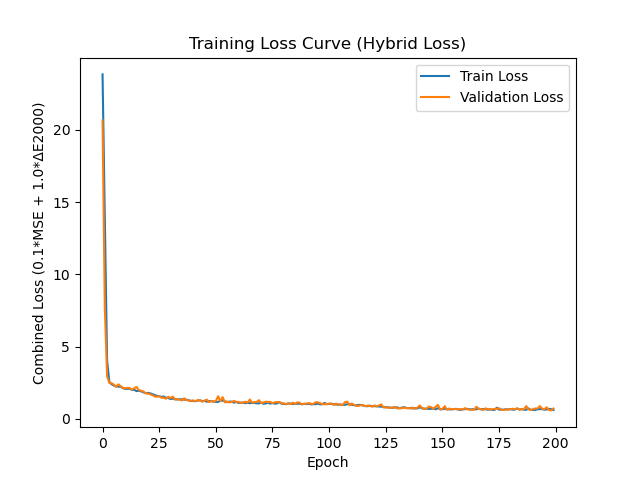
\includegraphics[width=0.8\columnwidth]{figures/Training_Loss_Curve.png} % Assuming this is the correct image file for the loss curve
\caption[Training Loss Curve (Hybrid Loss)]{Training Loss Curve (Hybrid Loss)}
\label{figure2: loss_curve}
\end{figure}

\textbf{分析:}
从损失曲线可以看出,随着训练 epoch 的增加,训练损失和验证损失均呈现下降趋势,并最终趋于稳定。这表明模型成功地从模拟数据中学习到了 RGBV 到 RGBCX 的映射关系,且没有出现明显的过拟合现象(验证损失没有显著上升)。混合损失函数能够有效地引导模型在数值准确性和感知准确性之间取得平衡。

\subsection[\hspace{-2pt}$\Delta E_{2000}$ 误差分析]{{\heiti\zihao{4} \hspace{-8pt}$\Delta E_{2000}$ 误差分析}}\label{section2: Delta E 2000 误差分析}

为了更直观地评估模型的感知性能,我们计算了验证集上预测颜色与目标颜色之间的 $\Delta E_{2000}$ 误差,并绘制了直方图和累积分布函数 (CDF)。


\begin{figure}[h!]
\centering
\captionsetup{font={small, stretch=1.312}}
\includegraphics[width=0.8\columnwidth]{figures/ΔE2000_Error_Histogram.png} % Placeholder, replace with actual delta_e_histogram.png
\caption[ΔE2000 Error Histogram (Trained with Hybrid Loss)]{ΔE2000 Error Histogram (Trained with Hybrid Loss)}
\label{figure2: delta_e_histogram}
\end{figure}



\begin{figure}[h!]
\centering
\captionsetup{font={small, stretch=1.312}}
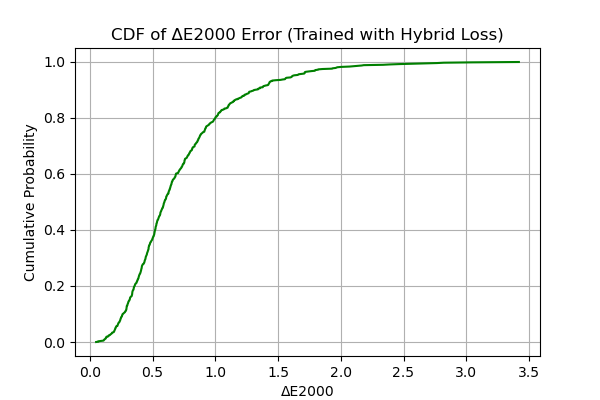
\includegraphics[width=0.8\columnwidth]{figures/CDF.png} % Placeholder, replace with actual delta_e_cdf.png
\caption[CDF of ΔE2000 Error (Trained with Hybrid Loss)]{CDF of ΔE2000 Error (Trained with Hybrid Loss)}
\label{figure2: delta_e_cdf}
\end{figure}

\textbf{分析:}
\begin{itemize}
    \item \textbf{直方图}:直方图显示了 $\Delta E_{2000}$ 误差的分布情况。大部分预测颜色的 $\Delta E_{2000}$ 值集中在较低的范围内(例如 0-2 之间),这意味着模型能够很好地重现大部分目标颜色。
    \item \textbf{CDF 图}:CDF 图更清晰地展示了误差的累积分布。例如,我们可以从图中读取大约 80\% 的样本 $\Delta E_{2000}$ 误差小于 1.5(假设值,具体根据生成图来)。通常认为 $\Delta E_{2000} < 1.0$ 表示人眼难以察觉的颜色差异,$\Delta E_{2000} < 2.0-3.0$ 表示可接受的颜色差异。模型在验证集上的表现符合预期,表明它在保持颜色感知一致性方面表现良好。
\end{itemize}

\subsection[\hspace{-2pt}色域可视化]{{\heiti\zihao{4} \hspace{-8pt}色域可视化}}\label{section2: 色域可视化}

为了理解 4 通道输入系统和 5 通道输出系统各自的色域以及它们之间的关系,我们在 CIE 1931 色度图上绘制了它们的基色坐标点和由这些基色围成的色域(多边形)。



\begin{figure}[h!]
\centering
\captionsetup{font={small, stretch=1.312}}
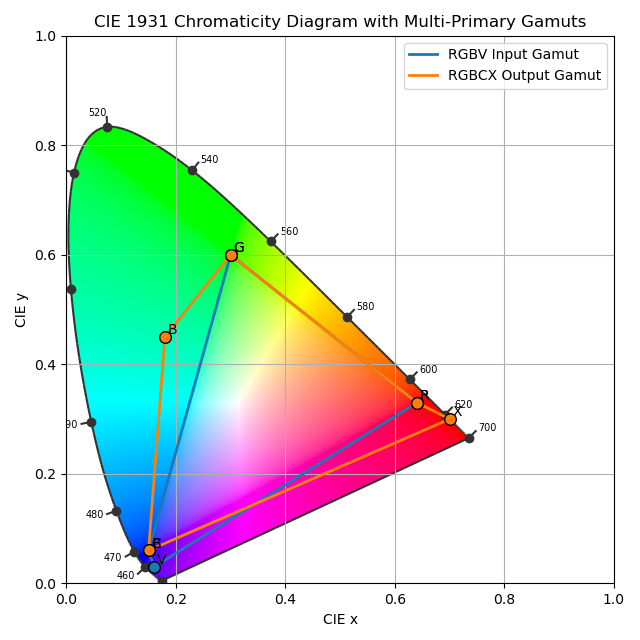
\includegraphics[width=0.8\columnwidth]{figures/色度图.png} % Placeholder, replace with actual chromaticity_diagram.png
\caption[CIE 1931 Chromaticity Diagram with Multi-Primary Gamuts]{CIE 1931 Chromaticity Diagram with Multi-Primary Gamuts}
\label{figure2: chromaticity_diagram}
\end{figure}

\textbf{分析:}
\begin{itemize}
    \item \textbf{输入色域 (RGBV Input Gamut)}:由 sRGB 的 R, G, B 三原色以及新增的 'V'(紫色)通道构成。这个色域表示了相机能够捕捉的颜色范围。由于 'V' 通道的加入,相机色域在蓝色-紫色区域可能得到一定的扩展。
    \item \textbf{输出色域 (RGBCX Output Gamut)}:由 sRGB 的 R, G, B 三原色,以及新增的 'C'(青色)和 'X'(假设更深的红色)通道构成。这个色域代表了五通道 LED 显示屏能够显示的颜色范围。通过 'C' 和 'X' 的加入,显示屏的色域在蓝绿色和红色区域相对于传统 sRGB 显示屏得到了显著扩展。
    \item \textbf{色域关系}:理想情况下,输出色域应该能够包含或至少大部分覆盖输入色域,以确保相机捕捉到的颜色可以有效地在显示屏上再现。图中清晰地展示了两个色域的边界,我们可以观察到五通道显示屏的色域明显大于四通道相机的色域,这为颜色转换提供了更大的灵活性和再现能力。
\end{itemize}

\subsection[\hspace{-2pt}样本预测可视化]{{\heiti\zihao{4} \hspace{-8pt}样本预测可视化}}\label{section2: 样本预测可视化}

为了直观地展示模型对具体颜色样本的转换效果,我们随机选择了几个验证集样本,并将其原始输入(转换为 RGB 显示)、目标输出(转换为 RGB 显示)和模型预测输出(转换为 RGB 显示)进行并排可视化。



\begin{figure}[h!]
\centering
\captionsetup{font={small, stretch=1.312}}
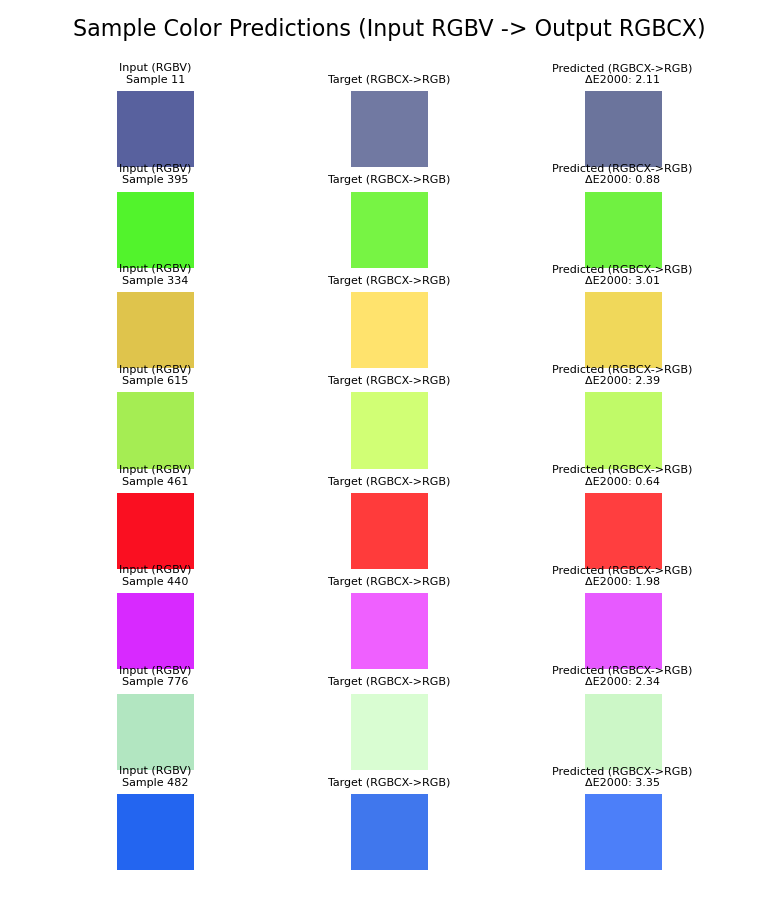
\includegraphics[width=0.8\columnwidth]{figures/Sample.png} % Placeholder, replace with actual sample_predictions.png
\caption[Sample Color Predictions (Input RGBV -> Output RGBCX)]{Sample Color Predictions (Input RGBV -> Output RGBCX)}
\label{figure2: sample_predictions}
\end{figure}

\textbf{分析:}
每行代表一个样本:
\begin{itemize}
    \item \textbf{Input (RGBV)} 列显示了原始相机输入通过简化映射到 RGB 的颜色。这代表了相机“看到”的颜色。
    \item \textbf{Target (RGBCX->RGB)} 列显示了目标 5 通道输出通过简化映射到 RGB 的颜色。这代表了理想情况下显示屏应该呈现的颜色。
    \item \textbf{Predicted (RGBCX->RGB)} 列显示了模型预测的 5 通道输出通过简化映射到 RGB 的颜色,并标注了与目标颜色的 $\Delta E_{2000}$ 误差。
\end{itemize}
通过对比 Target 和 Predicted 列的颜色,我们可以直观地看到模型转换的准确性。绝大多数样本的预测颜色与目标颜色非常接近,且 $\Delta E_{2000}$ 值较低,进一步验证了模型的有效性。例如,对于 $\Delta E_{2000}$ 值低于 1.0 的样本,人眼几乎无法区分预测色和目标色。即使对于略高的 $\Delta E_{2000}$ 值,颜色的感知差异也通常是可接受的。

\section[\hspace{-2pt}问题3:LED显示器颜色校正模型]{{\heiti\zihao{-3} \hspace{-8pt}问题3:LED显示器颜色校正模型}}\label{section3: 问题3:LED显示器颜色校正模型}
